\documentclass[12pt]{article}
\usepackage{setspace}
\usepackage{geometry}
\usepackage{hyperref}
\usepackage{multicol}
\usepackage{booktabs}
\usepackage{amssymb}
\usepackage{graphicx}
\usepackage{caption}
\usepackage{float}
\usepackage{setspace}
\usepackage{amsmath}
\usepackage{comment}




\geometry{margin=1in}
\bibliographystyle{plain}

\title{Determinants of Earnings Risk with Machine Learning}

\author{Ethan Ballou\thanks{University of Wisconsin - Milwaukee}}


\date{\today}

\begin{document}
\maketitle
\thispagestyle{empty}


%\date{\today}
%\pubMonth{Month}
%\pubYear{Year}
%\pubVolume{Vol}
%\pubIssue{Issue}
%\JEL{}
%\Keywords{}

\begin{abstract}
\begin{singlespace}


\noindent This paper looks at the determinants of lifetime earnings risk under a Restricted Income Profile (RIP) model using traditional and machine learning methods such as lasso and SHAP values. The paper builds on the work of Drewianka and Oberg (2025) which uses a moment condition approach derive a parameter that captures permanent income risk. The paper finds that education and age are important in explaining lifetime earnings risk. The paper also finds that macroeconomic variables such as probability of recession and real GDP growth are important and along with state controls may further imply a role of government policy. Finally, the paper finds that occupation controls are important while industry controls do not appear to play a strong role. 

\end{singlespace}
\end{abstract}


\vspace{1cm}

\noindent

\textbf{Keywords}: machine learning, restricted income profile, earnings instability, risk \\
\indent \textbf{JEL Codes}: D8, J0, D3\\




\clearpage
\setcounter{page}{1}












\begin{comment}


1.	Opening motivation
	•	Importance of understanding earnings risk for individual welfare and policy
	•	Distinction between annual vs. lifetime risk and why lifetime risk matters for major life choices
	2.	Classic RIP vs. HIP debate
	•	RIP (“Restricted Income Profile”) models assume homogeneous expected growth; HIP (“Heterogeneous Income Profile”) allow individual growth rates  
	•	Implications for estimated variance and persistence of earnings shocks
	•	Summary of Drewianka & Oberg (2025): moment-statistic approach to test for heterogeneity in profiles  
	3.	Literature on annual vs. lifetime earnings risk
	•	Annual-risk measures (e.g. Meghir & Pistaferri 2004) capture temporary vs. permanent shocks
	•	Previous work estimating lifetime risk (Drewianka & Oberg, “Heterogeneous Lifetime Earnings Risk”): formulas for present-value variance, empirical patterns  
	•	Gaps: annual moments and lifetime‐risk measures have not been fully integrated
	4.	Identification of the gap
	•	Neither RIP/HIP moment tests nor lifetime-risk measures alone address how profile heterogeneity affects lifetime risk
	•	Existing RIP/HIP tests focus on bias in σ²η but ignore full present-value implications
	•	Lifetime-risk studies allow heterogeneity in σ²η and θ but do not leverage moment-condition diagnostics
	5.	This paper’s contributions
	1.	Unify moment-statistic diagnostics (γ‐ and α‐based tests) with lifetime present-value framework
	2.	Extend RIP/HIP bias analysis to show how mis-specifying growth heterogeneity distorts lifetime risk estimates
	3.	Estimate a jointly-specified model of expected growth, σ²η(t), and σ²ν(t) across horizons to produce individual-level lifetime-risk measures
	4.	Empirical application to PSID 1970–2015: document how profile heterogeneity alters conventional lifetime-risk patterns
	6.	Key findings (brief)
	•	Moment-statistics show only modest heterogeneity in expected growth once autoregressive shocks are allowed
	•	Lifetime-risk estimates shift meaningfully when you incorporate profile heterogeneity diagnostics
	•	Behavioral validation: lifetime-risk better predicts major life decisions than annual-risk metrics
	7.	Roadmap of the paper
	•	Section 2: Theoretical framework—RIP/HIP specs, moment γ/α statistics, present-value formulas
	•	Section 3: Empirical strategy—PSID sample, construction of γ, α, and out-of-sample forecasts of σ²η, σ²ν, G(τ)
	•	Section 4: Intermediate results—patterns in annual growth and risks across cohorts, ages, controls
	•	Section 5: Main results—joint estimation of profile heterogeneity and lifetime-risk measures; bias diagnostics
	•	Section 6: Behavioral validation—predictive power for major decisions
	•	Section 7: Conclusion and policy implications




\end{comment}



% EDU1 - less than high school
% EDU2 - high school or some college
% EDU3 - bachelor's but less than master's




% mention how lasso weighs more heavily items with larger coefficents, where stepwise just cares about the p-value regardless of size.







\begin{onehalfspace}

\section{Introduction}

% motivation

Understanding the nature of earnings risk is central to both individual decision making and policy. People are often thought to be risk averse not risk neutral and therefore earnings risk has an effect on how individuals make intertemporal decisions such as saving. Especially on the analysis side, structural life cycle models have to make assumptions about the nature of earnings dispersion and risk. Misspecifying the earnings process can lead to inaccurate or incorrect conclusions in many cases and this is why understanding the nature of earnings risk and the earnings process is so important.

To better pin down the quantitative importance of shocks versus profile heterogeneity, this paper builds on the work of (Drewianka and Oberg 2025, 2019) \cite{drewianka2025,drewianka_oberg2019} which uses a moment condition approach to test for heterogeneity in expected income processes. The paper uses a Restricted Income Profile (RIP) model to estimate lifetime earnings risk and then tests for heterogeneity in expected income processes using a moment condition approach. 

Restricted Income Profile (RIP) models posit that all individuals with the same observed characteristics follow the same earnings trajectory. Deviations then being attributed to shocks to the individuals income process. In RIP, dispersion is then attributed to the variance of these shocks. (Abowd and Card, 1989; Meghir and Pistaferri, 2004) \cite{abowd_card1989,meghir_pistaferri2004} To appreciate the implications of these differing assumptions, it is helpful to compare RIP directly with HIP models. Heterogeneous Income Profile (HIP) models allow for different expected income processes for individuals with the same observed characteristics. This means that the variance of shocks is not the only source of dispersion in earnings. While some of the variance is due to shocks the rest of the variance is due to the different expected income processes. (Guvenen 2007; Baker 1997) \cite{guvenen2009,baker1997}Choosing between RIP and HIP can dramatically change the estimation of the variance of earnings shocks and hence change the estimation of earnings risk. 

This paper looks beyond that and tests for determinants of lifetime earnings risk as parameterized by the model in Drewianka and Oberg (2025) \cite{drewianka2025}. This paper finds that education and age are important in explaining lifetime earnings risk. The paper also finds that macroeconomic variables such as probability of recession and real GDP growth are important and play at least a small role and that the inclusion of state controls may further the hypothesis of government policy playing a role. Finally, the paper finds that occupation controls are important while industry controls do not appear to play a large role.



This paper contributes to multiple strands of literature. The first is the literature around (RIP) models and their use in life cycle models. (MaCurdy 1982; Abowd and Card 1989; Hryshko 2012). \cite{macurdy1982, abowd_card1989, hryshko2012} In addition to that it also contributes to a second strand of literature focusing on lifetime earnings risk. (Drewianka and Oberg 2025; Guvenen 2007; Meghir and Pistaferri 2004). \cite{drewianka2025,guvenen2007,meghir_pistaferri2004} Finally the paper contributes to the literature on machine learning and its use in economics by utilizing neural networks and SHAP values to interpret the results (Lundberg and Lee, 2017). \cite{lundberq} 

The rest of the paper is structured as follows. Section 2 discusses the model and data, Section 3 discusses the empirical strategy, Section 4 discusses the results, and Section 5 concludes the paper. 

\section{Data and Model}

As mentioned before, the model used is the same model from Drewianka and Oberg (2025) \cite{drewianka2025}. The model is a standard RIP model where people's income are modeled as a function of characteristics, but where there are no individual level effects. Then each individual has a deviation from the expected income process which is modeled as a shock. For example all 22 year old men from the US will have the same expected income process based off of those characteristics. However their actual income will deviate from this expected income process due to shocks. 
\vspace{-0.75cm} % Adjust the value as needed to reduce spacing
\begin{align}
u_{it} 
&= \pi_{it} + \nu_{it} \\[1ex]
\pi_{it} 
&= \rho\,\pi_{i(t-1)} + \eta_{it},
\end{align}

\vspace{-0.25cm}

$u_{it}$ is the shock or deviation from the expected income process for a given person i in time t. This process of shocks can be decomposed into two types of shocks: persistent and temporary shocks as outlined in equation 1. $\pi_{it}$ is the cumulative effect from the persistent shocks which are further modeled in equation 2 while $\nu_{it}$ are the temporary shocks. The temporary shocks along with $\eta_{it}$ are assumed to be mean zero and independent across individuals and time. The persistent shocks are further modeled as an autoregressive process with $\rho$ being the persistence of the shocks and $\eta_{it}$ being the actual shock.

To get a measure of earnings risk the variance of $\eta_{it}$ across time is calculated. This is capturing the correlation of permanent income shocks across time for each individual. To calculate this the following equation is used:

\vspace{-0.75cm}

\begin{align}
\Omega_i(t,t+k)
&\equiv u_{i(t+k)} - u_{it}\\[1ex]
\Omega_i(t,t+k)
&= \nu_{i(t+k)} - \nu_{it}
  + \sum_{j=1}^k \eta_{i(t+j)}.
\end{align}

\vspace{-0.25cm}

This omega equation differences $u_{it}$ across a window t to t+k. This is then multiplied by another omega function across the window t-j to t+k+q. This will result in the persistent shocks in the interval (t, t+k) showing up twice while the other persistent shocks don't necessarily show up twice. This results in the variance of the shocks across time k as follows:

\vspace{-0.5cm}

\begin{gather}
E\Bigl[\tfrac{1}{k}\,\Omega_i(t,t+k)\,\Omega_i(t-j,t+k+q)\Bigr]
= \sigma^2_{\eta_i},\\
\gamma_{itjq}
\equiv \tfrac12\,\Omega_i\bigl(t,\,t+2\bigr)\,\Omega_i\bigl(t - j,\,t + 2 + q\bigr).
\end{gather}

This is then further used to get the following moment condition for the variance of $\eta_{it}$ that is a function of (j+k+q) and j and can be estimated in a regression framework to get a measure of lifetime earnings risk $\gamma_{itjq}$. For more on the derivation see Drewianka and Oberg (2025) \cite{drewianka2025}:

\vspace{-0.75cm}

\begin{align}
E[\gamma_{itjq}]
&\approx
\bigl[\delta^2\,E\pi^2_{i(t-j)}\,(j+k+q)\bigr]
- \bigl[\delta\,s_i(t-j+1,t)\,j\bigr]
+ \bigl[\sigma^2_{\eta_i(t+1)}
  - \delta\,\sigma^2_{\eta_i(t+1)}\,(k+q)\bigr] \\[1ex]
E[\gamma_{itjq}]
&=
\sigma^2_{\eta_i(t+1)}
+ \bigl[\delta^2\,E\pi^2_{i(t-j)} - \delta\,\sigma^2_{\eta_i(t+1)}\bigr]\,(j+k+q)
+ \delta\,\bigl[\sigma^2_{\eta_i(t+1)} - s_i(t-j+1,t)\bigr]\,j
\end{align}

The data used is the 1970-2015 waves of the Panel Study of Income Dynamics (PSID 2017). \cite{psid2017} The sample is of men between the ages of 22 and 69 with students being excluded. Many of the men in the sample come from the Survey of Economic Opportunity which has been shown to be representative of the main PSID sample (SEO; Hill 1992; Drewianka 2010). \cite{hill1992, drewianka2010} Income is calculated in 2015 dollars using the Consumer Price Index (CPI 2017). \cite{cpi2017} The analysis uses several key variables, including education (categorized as less than high school, high school or some college, and bachelor's degree but less than a master's degree), age (with higher-order polynomial terms Age$^2$ and Age$^3$ to capture non-linear effects), and macroeconomic indicators such as the probability of a recession (P(Recession)) and real GDP growth. Individual-specific variables include fixed effects for wages, a moving average of income over the last five years (MA(Last 5 years income)), employment status (Employed), veteran status (Veteran), and job tenure (years in the current job). The primary outcome variable, gamma ($\gamma$), measures lifetime earnings risk derived from the variance of persistent income shocks. Additionally, the analysis incorporates fixed effects for occupation, industry, state of residence, and other controls such as year, race, and cohort. With the theoretical framework and data laid out, the following section turns to the empirical implementation of the model.

% define variables used?

\section{Empirical Strategy}

The empirical strategy of this paper is broken into two parts. The first part is estimating gamma and then constructing a weighted gamma for each individual in each year since gamma alone is across i, t, j, and q. (i - individual, t - time, j and q - period or "window" used in calculation of gamma). The second part of the empirical strategy is estimating the then weighted gamma variable using various models and variables to look for trends in the characteristics of individuals in regards to lifetime earnings risk.

For the estimation of gamma and consolidation across j and q is done by using a mixed regression for the gamma and then a fixed effects regression to get the composite or weighted gamma for each person year.

The following mixed regression is used to estimate gamma based on the above equation. This is done to get an estimate of gamma for each individual in each year across j and q. A mixed regression used instead of standard OLS because $\sigma^2_{\eta_i}$ is correlated with both the constant and the coefficient on (j+k+q) as seen in equation 8 and therefore a mixed regression is used to account for this by allowing the residuals to be separately correlated with (j+k+q) for each individual i in year t. (For more on this see Drewianka and Oberg (2025) \cite{drewianka2025}) The mixed regression is as follows:


\vspace{-0.75cm}



\begin{align}
\gamma_{itjq}
&= \beta_{0}
  + \beta_{1}\,(j + k + q)
  + \beta_{2}\,j
  + \epsilon_{itjq}, \\[1ex]
\epsilon_{itjq}
&= \beta_{0it}
  + \beta_{1it}\,(j + k + q)
  + e_{itjq}.
\end{align}

The random effects component (j+k+q) models how each person-year combination may have a unique relationship with the (j+k+q) variable while the cov(unstructured) option in Stata allows for unrestricted correlation between the random intercept and slope. The standard errors are clustered at the person level to account for within-person correlation across time.

From here a regression is run across fixed effects for each combination of j and q with year effects absorbed. Weights are then calculated for each combination of j and q based on their accuracy in predicting gamma using inverse MSE. Specifically, after estimating the fixed effects model, the mean squared residual (MSE) is calculated for each (j,q) combination, then use the square root of the inverse of these values ($\sqrt{(1/MSE)}$) as weights. Then the weighted gamma is calculated consolidating across j and q so that there are only individual-year gamma values. Having obtained individual-year estimates of earnings risk, we now examine the determinants of this risk using several regression techniques.

The second part of the empirical strategy uses various models to estimate lifetime earnings risk (gamma). We begin with the simplest specification to establish a baseline before introducing more sophisticated selection and machine-learning methods. The first model is a standard OLS regression of the lifetime earnings risk variable, gamma, on various controls and variables. The second model is a stepwise regression which selects variables based on a p-value threshold. The third model is a lasso regression which penalizes the size of the coefficients to select variables. Finally, the fourth model uses a multi-layer perceptron and SHAP values to interpret the results.

The OLS regressions are fairly standard however the stepwise and lasso models do have components that are worth mentioning. For the stepwise regression model a cutoff p-value of 0.05 is used to select variables. The model removes the least significant variable (or group of variables in the case of a set of controls) in rounds until it reaches the cutoff. 0.05 was selected so that the model would still select some variables but the rankings of the many of the variables would be clear. A higher cutoff and most of the variables would be selected and cardinal rankings would not be visible. Too low of a cutoff value and many of the variables would not be selected at all. 

As for the lasso model, the model is set up to select variables based on the Bayesian Information Criterion (BIC) which is a common method for selecting variables in penalized regression. While the model selects lambda based on cross-validation, the selected model isn't very relevant to the analysis as the rankings are so the selected model isn't discussed. It is worth mentioning however that the lasso model is a penalized regression and therefore some weight is assigned to the size of the coefficients when selecting variables. This is different from the stepwise regression which is indiscriminate regarding the size of the coefficient and only considered the significance of a variable.

Finally the multi-layer perceptron model is a neural network that is used to estimate lifetime earnings risk. The model is trained on the same variables and data used by the OLS, stepwise, and lasso models. The model is 4 dense layers (excluding the input layer) with 1000 nodes each and a linear output layer at the end. The model used a sigmoid activation function in the hidden layers to allow for continuous support. This was done instead of a ReLU activation function to allow for more definition in the parameters instead of some parts of the perceptron being "dead" and not contributing and complicating the SHAP value interpretation. This model size and structure was selected as it achieved the best performance in terms of mean squared error (MSE). The model trained with MSE as its loss function and used early stopping to prevent overfitting and trained on 70 percent of the data with the rest being used for test and validation.

The SHAP values are then used to interpret the results of the multi-layer perceptron model. SHAP values are constructed by calculating marginal contribution of a variable as a deviation from the output variable's mean if the variable was changed. This is done across a sample of observations and gives each variable a distribution of SHAP values. The summary plot shows the distribution of SHAP values for the continuous variables. 

\section{Results}

% does the sign matter? Address this 


\begin{figure}[H]
    \centering
    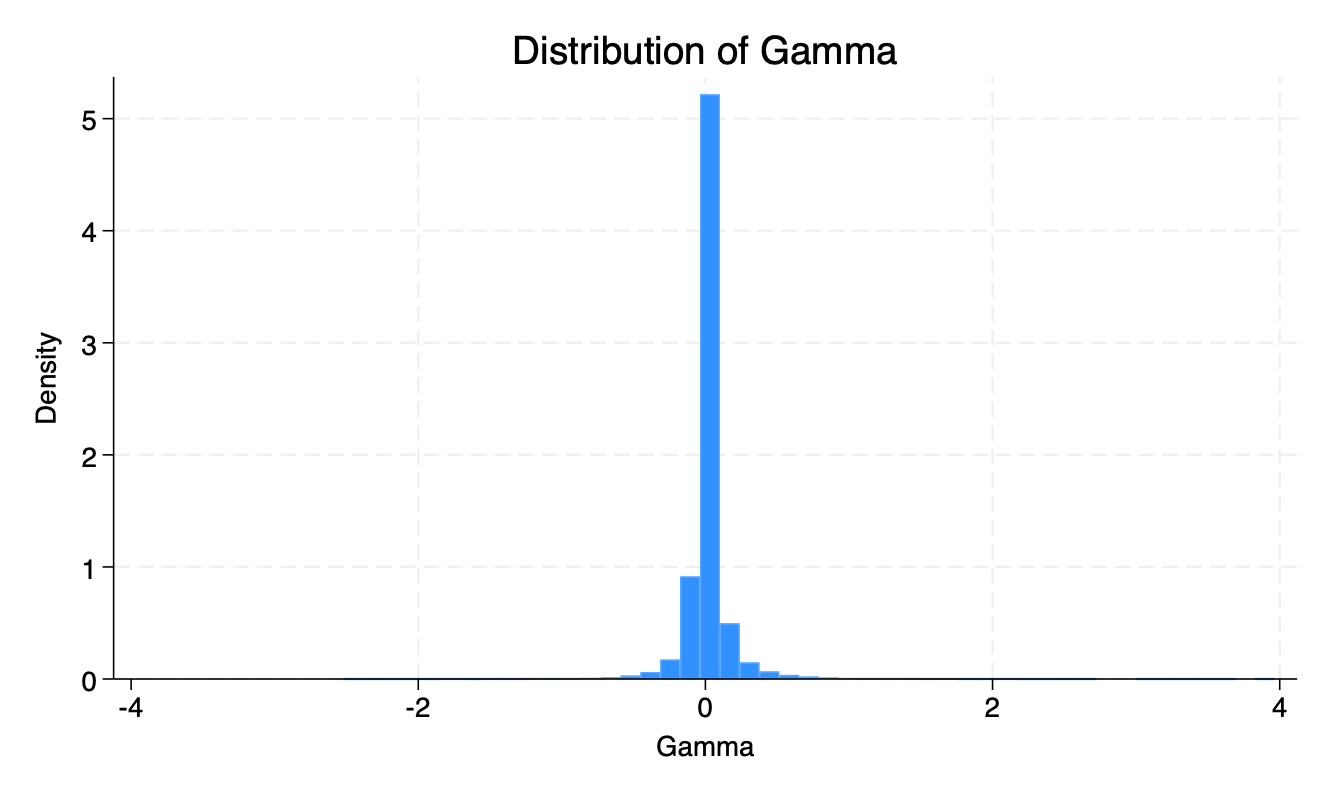
\includegraphics[width=.7\textwidth]{/Users/ethanballou/Documents/GitHub/LifetimeEarningsRisk/Plots/Graph2.png}
    \caption{Distribution of Gamma}
\end{figure}






Gamma is a centered heavily around 0 with a standard deviation of 0.1686 as seen in Figure 1. Being centered at 0 is due to its derivation and as seen in Figure 2 there is not a clear correlation with age which might be expected. However there does seem to be a slight tightening past the age of 60 as the variance of gamma appears to decrease at least somewhat. To formally quantify these patterns, we next present regression estimates of gamma across several specifications.



\begin{figure}[H]
    \centering
    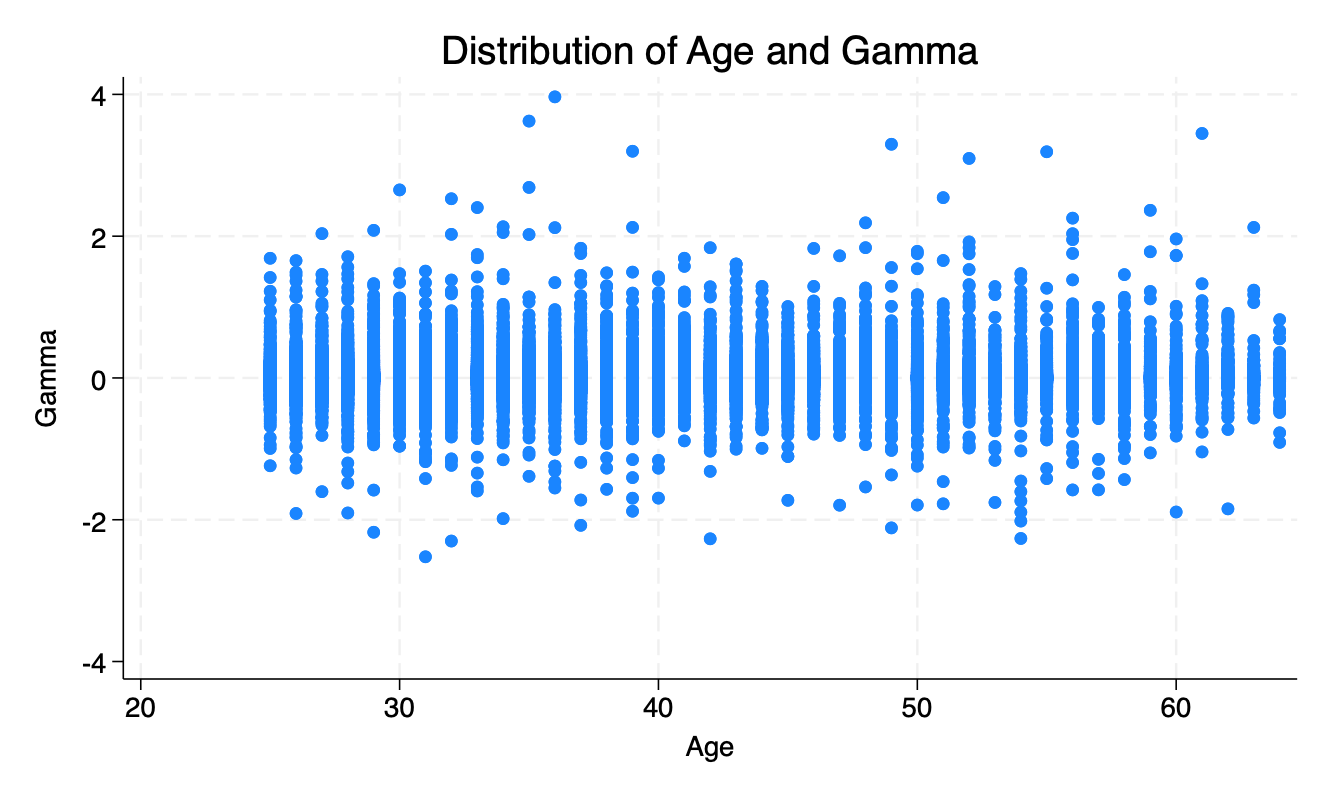
\includegraphics[width=.7\textwidth]{/Users/ethanballou/Documents/GitHub/LifetimeEarningsRisk/Plots/Graph1.png}
    \caption{Scatterplot of Age vs. Gamma}
\end{figure}






\end{onehalfspace}


\begin{table}[H]
\centering
\caption{OLS Estimates for $\gamma$ (Coefficients $\times$ 100)}

\begin{tabular}{lccccc}

\toprule
                    & (1)     & (2)   & (3)    & (4)      & (5)         \\
\midrule
Education (less than 12)                & $-0.361$  & $-0.360$    & $-0.522^{*}$  & $-0.597^{*}$   & $-0.630^{**}$    \\
                    & (0.255)   & (0.273)     & (0.286)   & (0.307)    & (0.310)     \\
Education (12 to 14)                & $-0.283$  & $-0.315^{*}$    & $-0.418^{**}$  & $-0.417^{*}$   & $-0.455^{**}$    \\
                    & (0.175)   & (0.181)     & (0.193)   & (0.216)    & (0.219)     \\
Education (14 to 16)                & $-0.089$  & $-0.063$    & $-0.138$  & $-0.114$   & $-0.147$    \\
                    & (0.206)   & (0.209)     & (0.216)   & (0.228)    & (0.230)     \\
P(Recession)            & $-0.006$   & $-0.038$     & $-0.037$   & $-0.040$    & $-0.039$     \\
                    & (0.005)   & (0.036)     & (0.036)   & (0.036)    & (0.036)     \\
Real GDP Growth            & $-0.033$   & $0.076$     & $0.071$   & $0.063$    & $0.058$     \\
                    & (0.033)   & (0.172)     & (0.172)   & (0.172)    & (0.172)     \\
Fixed Effect for Wage         & $-0.006$   & $0.004$     & $0.005$   & $0.002$    & $0.004$     \\
                    & (0.025)   & (0.027)     & (0.027)   & (0.028)    & (0.028)     \\
MA(Last 5 years income)              & $0.004$   & $0.003$     & $0.004$   & $0.004$    & $0.004$     \\
                    & (0.003)   & (0.003)     & (0.003)   & (0.003)    & (0.004)     \\
Veteran             & $0.021$   & $-0.003$     & $0.053$   & $0.018$    & $0.040$     \\
                    & (0.141)   & (0.151)     & (0.153)   & (0.154)    & (0.155)     \\
Employed                 & $0.627$   & $0.584$     & $0.550$   & $0.619$    & $0.625$     \\
                    & (0.627)   & (0.628)     & (0.628)   & (0.629)    & (0.629)     \\
Job Tenure              & $-0.010$   & $-0.009$     & $-0.008$   & $-0.012$    & $-0.010$     \\
                    & (0.011)   & (0.012)     & (0.012)   & (0.012)    & (0.012)     \\
Age          & $0.874^{**}$   & $0.936^{**}$     & $0.926^{**}$   & $0.919^{**}$    & $0.907^{**}$     \\
                    & (0.380)   & (0.384)     & (0.385)   & (0.385)    & (0.385)     \\
Age$^2$        & $-0.023^{**}$  & $-0.025^{***}$    & $-0.025^{***}$  & $-0.025^{***}$   & $-0.024^{***}$    \\
                    & (0.009)   & (0.009)     & (0.009)   & (0.009)    & (0.009)     \\
Age$^3$      & $0.0002^{***}$  & $0.0002^{***}$    & $0.0002^{***}$  & $0.0002^{***}$   & $0.0002^{***}$    \\
                    & (0.0001)   & (0.0001)     & (0.0001)   & (0.0001)    & (0.0001)     \\

\midrule
Occupation Controls  &               &                 &               & \checkmark    & \checkmark     \\
Industry Controls    &               &                 & \checkmark    &               & \checkmark     \\
Other Controls      &               & \checkmark      & \checkmark    & \checkmark    & \checkmark     \\
\midrule
Observations        & 62,900        & 62,900          & 62,900        & 62,900        & 62,900         \\
\bottomrule
\end{tabular}%
\newline
\textit{Notes:} Standard errors in parentheses. Other controls include state, year, race, and cohort fixed effects. Statistical significance: $^{*}p<0.10$, $^{**}p<0.05$, $^{***}p<0.01$. All coefficients and standard errors are multiplied by 100 for easier interpretation.

\end{table}

\begin{onehalfspace}

% EDU3 and industry interaction? FE regression with industry controls and industry controls with EDU3 interaction


The beginning of the analysis is just simple OLS regressions of gamma. The further analysis will focus on which variables are most significant or important and less on the actual size of the effect. However size of coefficients is something OLS can easily address. While gamma is centered around zero, variables do still have effects despite being small. Table 1 shows the OLS estimates for gamma across different specifications. The different specifications include different sets of controls, such as occupation and industry controls along with other controls such as state, year, cohort, and race.


The coefficients are quite small however some are larger than others. Less than high school and high school or some college education are lightly significant in some cases. They have some of the larger effects compared to many of the variables with less than high school being somewhere around -0.004 and -0.006 and high school and some college being around -0.003 to -0.005. 

The bachelor's degree and less than a master's variable is smaller than the other two education variables which would imply college education does provide stabler employment and earnings overall. However despite this the variable is not significant in any of the models suggesting larger variation in earnings for those with a bachelor's degree or less than a master's degree. This variation could be due to variation in fields of study which would explain the larger coefficients in models 3, 4, and 5 where industry or occupation controls are included.


The other variables that are significant are the age variables. The age, age squared, and age cubed variables are all significant in all models. The interesting result is that the age squared and cubed variables are slightly more significant than the regular age variable. On some level it is expected that towards the end of a person's career they would become more risk averse and it is possible the squared and cubed terms capture this variation occurring right before retirement. Overall the OLS results show that education and age are important in explaining lifetime earnings risk. This pattern continues in the stepwise and lasso results.



\end{onehalfspace}


\begin{table}[H]
\centering
\caption{Stepwise Cardinal Ranking of Importance Results for $\gamma$}

\begin{tabular}{lccccc}

\toprule
                    & (1)     & (2)   & (3)    & (4)      & (5)         \\

\midrule
Education (less than 12)                & selected  & 2    & 2  & selected   & selected    \\
Education (12 to 14)                & selected  & 1    & 1  & selected   & selected    \\
Education (14 to 16)                & 6  & 10    & 8  & 6   & 6    \\
P(Recession)             & 1   & 3     & 3   & 1    & 1     \\
Real GDP Growth            & 4   & 4     & 4   & 4    & 4     \\
Fixed Effect for Wage         & 7   & 11     & 13   & 9    & 9     \\
MA(Last 5 years income)              & 2   & 6     & 6   & 3    & 3     \\
Veteran             & 8   & 12     & 12   & 10    & 11     \\
Employed                 & 3   & 5     & 5   & 2    & 2     \\
Job Tenure               & 5   & 7     & 9   & 5    & 5     \\
Age          & selected   & selected     & selected   & selected   & selected     \\
Age$^2$        & selected  & selected    & selected  & selected   & selected    \\
Age$^3$      & selected  & selected    & selected  & selected   & selected    \\

\midrule
Occupation Controls      & -   & -    & -  & selected   & selected    \\
Industry Controls      & -  & -    & 7  & -   & 10    \\
Cohort Controls      & -  & 8    & 10  & 7   & 7    \\
Race Controls      & -  & 13    & 14  & 11   & 12    \\
Year Controls      & -  & 9    & 11  & 8   & 8    \\
State Controls      & -  & selected    & selected  & selected   & selected    \\

\midrule
Occupation Controls  &               &                 &               & \checkmark    & \checkmark     \\
Industry Controls    &               &                 & \checkmark    &               & \checkmark     \\
Other Controls      &               & \checkmark      & \checkmark    & \checkmark    & \checkmark     \\
\midrule
Observations        & 62,900        & 62,900          & 62,900        & 62,900        & 62,900         \\
\bottomrule
\end{tabular}%
\newline

\footnotesize
\textit{Notes:} This table reports results from stepwise regression models using a p-value threshold of 0.05. "Selected" indicates variables retained in the final model. Numbers indicate the order of variable removal (with 1 being the last variable removed before model finalization). "-" indicates the variable was not included in the initial model specification.

\end{table}


\begin{onehalfspace}


Table 2 shows the stepwise results for the same 5 models. The stepwise results are based on a p-value threshold of 0.05. The stepwise regression results are able to assign cardinal rankings to how significant certain variables are in explaining lifetime earnigns risk. In the stepwise regression the controls are treated as groups of variables such that the model cannot remove single variables from a set of controls and must remove the entire set of controls at once. The numbers assigned to the variables not selected indicate the order in which they were removed such that 1 is the last variable removed before the model is finalized.

The stewise regression results show similar results to OLS in that both education and age play an important role in predicting lifetime earnigns risk. Simlar to OLS less than highschool and high school and some college are the two education variables important to the model while the bachelors degree and less than a masters is not selected and not relevant in the model. And for the two models where the two important education variables aren't selected they are still the last two variables to be removed before the cutoff. 

The other interesting variables that show up are the probability of recession and real GDP growth. These two variables are in the last 4 variables to be removed in all models suggesting their importance. Specifically probability of recession was the last variable removed in 3 of the models despite different controls. Probability of recession and real GDP growth were both important with and without industry controls which would be where one would expect at least some of their variation to be captured. This implies that variation across industry sensitivity to macroeconomic outcomes may not actually have much explanatory power in lifetime earnings risk.

Some surprising results regarding items not in the model is that industry controls are not selected by the stepwise regression in either of the models it is included in. This is despite the third model not even including occupation controls. Not only are industry controls not selected they are not close to the cutoff either, being the 7th and 10th variable from the cutoff in the two models. This can be contrasted with state controls which are slected in every model. The inclusion of state controls along with the importance of probability of recession and GDP growth may suggest that government policy plays an important role in lifetime earnings risk. However if this were the case industry level policy does not seem to be a part of the mechanism, as varaition in industry policy within states would be captured by the industry controls.

Finishing up the controls, occupation and state controls are selected in all models where they are included. This is in contrast to the rest of the controls being far from the cutoff and not seen as relevant in the analysis. The interpretation of state controls could a couple of things. The first was already mentioned in the previous paragraph regarding variation in government policy across states. However the second interpretation would be that the labor market enviroment is significnatly different across states and this is being captured. While the labor market enviorment is heavily connected to governemnt policy, there are other factors that play a role. Labor markets are going to vary across states due to things like population density, resources, and other factors that are not directly related to government policy. In regard to occupation controls this is not very surprising as variation across job characteristics like qualifications, respoonsibilties and so forth is quite large even when considering within state and industry.

All in all the stepwise results show that education and age are important in explaining lifetime earnings risk. The stepwise results also show that macroeconomic variables such as probability of recession and real GDP growth are important and that the inclusion of state controls may further the hypothesis of government policy playing a large role. And finally the stepwise results show that occupation controls are important while industry controls do not appear to play a large role.


\end{onehalfspace}


\begin{table}[H]
\centering
\setlength{\tabcolsep}{3pt} % Adjust column spacing
\renewcommand{\arraystretch}{1} % Adjust row spacing
\caption{Lasso Cardinal Ranking of Importance Results for $\gamma$}

\begin{tabular}{lccccc}

\toprule
                    & (1)     & (2)   & (3)    & (4)      & (5)         \\

\midrule
Education (less than 12)                &  3  &  3    &  2  &  1   &  1    \\
Education (12 to 14)                &  2  &  1    &  1  &  1   &  1    \\
Education (14 to 16)                &  8  &  7    &  6  &  6   &  4    \\
P(Recession)             &  4    & Not Selected    & Not Selected   & Not Selected    & Not Selected     \\
Real GDP Growth            &  6    & Not Selected     & Not Selected   & Not Selected    & Not Selected     \\
Fixed Effect for Wage         &  7   &  9     &  9   &  8    &  6     \\
MA(Last 5 years income)              &  1   &  2     &  1   &  2    &  1     \\
Veteran             &  10   &  8     &  8   &  7    &  5     \\
Employed                 &  3   &  2     &  3   &  1    &  1     \\
Job Tenure               &  5   &  4     &  4   &  3    &  2     \\
Age          &  9   &  6     &  7   &  5    &  4     \\
Age$^2$        &  11  &  10    &  10  &  8   &  7    \\
Age$^3$      &  2  &  5    &  5  &  4   &  3    \\

\midrule
Occupation Controls      & -   & -    & -  & Selected   & Selected    \\
Industry Controls      & -  & -    & Selected  & -   & Selected    \\
Cohort Controls      & -  & Selected    & Selected  & Selected   & Selected    \\
Race Controls      & -  & Selected    & Selected  & Selected   & Selected    \\
Year Controls      & -  & Selected    & Selected  & Selected   & Selected    \\
State Controls      & -  & Selected    & Selected  & Selected   & Selected    \\


\midrule
Occupation Controls  &               &                 &               & \checkmark    & \checkmark     \\
Industry Controls    &               &                 & \checkmark    &               & \checkmark     \\
Other Controls      &               & \checkmark      & \checkmark    & \checkmark    & \checkmark     \\
\midrule
Observations        & 62,900        & 62,900          & 62,900        & 62,900        & 62,900         \\
\bottomrule
\end{tabular}%
\newline

\footnotesize
\textit{Notes:} This table reports variables selected by Lasso regression with Bayesian Information Criterion (BIC) variable selection. "Selected" indicates variables retained in the final model. Numbers in parentheses indicate the order in which variables were added to the model across variation in lambda. "-" indicates the variable was not included. "Not Selected" indicates the variable was not selected by Lasso for any lambda used in cross validation but was provided in the model specification.

\end{table}

\begin{onehalfspace}

% report mse or r2


Now moving on to the lasso results shown in Table 3. As mentioned before lasso is a penalized regression and tries to force coefficients to zero. This means lasso gives some weight to the size of the coefficients (relatively speaking) compared to stepwise which cares only about the p-value. The first point to be made is that all the controls are selected in all cases. The configuration of this lasso model is the same as the stepwise model in that it can either include an entire set of controls or none of them. 

Moving on from the controls, the two education variables that were important in the stepwise and OLS models are ranked quite high in importance as they were in the top three variables in every case. This continues the pattern of the less than high school and high school or some college variables playing an important role while the bachelor's degree and less than a master's variable is not as relevant. 

However one pattern that does break here is the age variables. The age variables are among the least relevant variables in this analysis. Particularly the age squared variable which is often one of the last variables selected by the model. This is in contrast to the OLS results where the higher order age variables were slightly more significant than the regular age variable. The hypothesis there being that these higher order age terms are capturing a decrease in variation right before retirement. However in the lasso models this is not the case when it comes to the age squared variable. However it could be that this variation is better captured in the age cubed variable which is seen as more important than even the regular age variable in 3 of the models.







\begin{figure}[H]
    \centering
    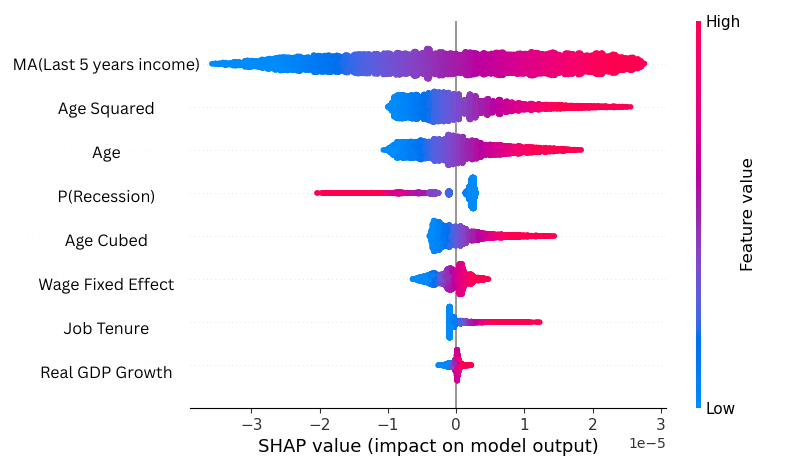
\includegraphics[width=1\textwidth]{/Users/ethanballou/Documents/GitHub/LifetimeEarningsRisk/Plots/SHAPsummaryPLOT_Edit.png}
    \caption{SHAP Summary Plot}
\end{figure}

\vspace{1cm}

The other observation to be made is regarding the probability of recession and real GDP growth variables. These two variables are not selected in any of the models except for the first model. This is in contrast to the stepwise results where they were both important. To complement the insights from penalized regression, we turn to a non-linear model interpretation via SHAP values.



Finally a summary of the shapley values are shown in Figure 3. This can add some detail to the analysis that linear models cannot by representing the effects of a variable not in a scalar way but in a distributional way.


The table shows just the continuous (or at least somewhat continuous) variables. Tenure, wage, and real GDP growth are shown to have relatively small effects regardless of the values. However the age variables display an interesting pattern. First the values are distributed such that lower values have a negative effect on gamma. However the more interesting observation is the skewness. All of the variables are skewed to the right as based on this for the really high values of age (which show up less often) the effect is positive. This is in contrast to the hypothesis that higher age may be related to a decrease in risk before retirement. However this is supported by the OLS results somewhat in that the cubed age variable was positive and very significant. That being said, based on the table the age squared variable has the most variation in effects compared to the rest of the age variables which does still support the result that age becomes important towards the end of a person's career. In the next section, we synthesize these findings and discuss their broader implications for understanding lifetime earnings risk.

%OCCUPATION AND INDUSTRY RESULTS


%Throughout all the analysis occupation controls were included in every possible model. These occupations and industries are now further analyzed in Tables 4 and 5. The results are shown in a similar way to the previous tables by ranking the variables. The LASSO ranking is based on the order in which variables would enter the model if the penalty were relaxed (across values of lambda) and the SHAP ranking is based on the importance of the variable in predicting lifetime earnings risk.


%\vspace{2cm}

\section{Conclusion}





To conclude the analysis, the results show that education and age are important in explaining lifetime earnings risk. The stepwise and lasso results show that macroeconomic variables such as probability of recession and real GDP growth are important and that the inclusion of state controls may further the hypothesis of government policy playing a large role. Finally, the stepwise results show that occupation controls are important while industry controls do not appear to play a large role.

Some limitations of the analysis are that the data is only men and that a household level model may be able to give more insight into the mechanisms at play. The data is also only from the PSID which may not be representative of the entire population. 

Some areas for further analysis whether in an estimation or life cycle structural way would be to look at the interaction of education and occupation or even occupation with some macroeconomic variables. It seems that macroeconomic variables play at least some small role depending on the controls included suggesting that an interaction with the controls may lend some insight into the mechanisms at play.






\end{onehalfspace}







\vspace{13cm}










\begin{comment}




\begin{table}[H]
\centering
\caption{Lasso and SHAP Results for Occupations}

\footnotesize  % Controls the font size of the table content

\begin{tabular}{lcc|lcc}
\toprule
Occupation & SHAP Rank & LASSO Rank & Occupation & SHAP Rank & LASSO Rank \\
\midrule
occ\_21 & 1 & Not Selected & occ\_60 & 2 & 16 \\
occ\_84 & 3 & 26 & occ\_61 & 4 & 13 \\
occ\_1 & 5 & 14 & occ\_45 & 6 & 20 \\
occ\_70 & 7 & Not Selected & occ\_98 & 8 & 14 \\
occ\_37 & 9 & Not Selected & occ\_97 & 10 & 27 \\
occ\_2 & 11 & 20 & occ\_99 & 12 & 22 \\
occ\_13 & 13 & 14 & occ\_9 & 14 & 24 \\
occ\_11 & 15 & 23 & occ\_83 & 16 & 21 \\
occ\_4 & 17 & 3 & occ\_101 & 18 & Not Selected \\
occ\_95 & 19 & 25 & occ\_79 & 20 & 15 \\
occ\_85 & 21 & Not Selected & occ\_6 & 22 & 8 \\
occ\_999 & 23 & Not Selected & occ\_8 & 24 & Not Selected \\
occ\_93 & 25 & 17 & occ\_55 & 26 & 21 \\
occ\_20 & 27 & 16 & occ\_53 & 28 & 23 \\
occ\_17 & 29 & 6 & occ\_19 & 30 & Not Selected \\
occ\_5 & 31 & 18 & occ\_40 & 32 & 23 \\
occ\_58 & 33 & 26 & occ\_34 & 34 & 19 \\
occ\_59 & 35 & 13 & occ\_7 & 36 & Not Selected \\
occ\_77 & 37 & 21 & occ\_87 & 38 & 21 \\
occ\_50 & 39 & 19 & occ\_14 & 40 & Not Selected \\
occ\_54 & 41 & 28 & occ\_96 & 42 & 15 \\
occ\_38 & 43 & 20 & occ\_3 & 44 & 12 \\
occ\_15 & 45 & 14 & occ\_32 & 46 & 14 \\
occ\_18 & 47 & 11 & occ\_42 & 48 & 11 \\
occ\_73 & 49 & Not Selected & occ\_31 & 50 & Not Selected \\
occ\_62 & 51 & 21 & occ\_44 & 52 & 17 \\
occ\_33 & 53 & 19 & occ\_63 & 54 & 28 \\
occ\_49 & 55 & 18 & occ\_86 & 56 & 17 \\
occ\_36 & 57 & Not Selected & occ\_43 & 58 & 16 \\
occ\_39 & 59 & Not Selected & occ\_74 & 60 & 17 \\
occ\_72 & 61 & Not Selected & occ\_64 & 62 & 2 \\
occ\_56 & 63 & Not Selected & occ\_92 & 64 & Not Selected \\
occ\_80 & 65 & Not Selected & occ\_88 & 66 & 13 \\
occ\_12 & 67 & 14 & occ\_75 & 68 & 25 \\
occ\_81 & 69 & Not Selected & occ\_30 & 70 & Not Selected \\
occ\_35 & 71 & 9 & occ\_57 & 72 & Not Selected \\
occ\_89 & 73 & Not Selected & occ\_71 & 74 & Not Selected \\
occ\_16 & 75 & 29 & occ\_94 & 76 & 25 \\
occ\_82 & 77 & Not Selected & occ\_52 & 78 & Not Selected \\
\bottomrule
\end{tabular}%
\newline

\footnotesize
\textit{Notes:} This table reports occupations selected by Lasso regression with Bayesian Information Criterion (BIC) for predicting earnings risk. "SHAP Rank" shows the variable importance ranking based on SHAP values (lower numbers indicate greater importance). "LASSO Order" indicates the order in which variables would enter the model if the penalty were relaxed. Note that the BIC-optimal model contained no occupation variables.

\end{table}





\begin{table}[H]
\centering

\caption{Lasso and SHAP Results for Industries}

\begin{tabular}{lcc}

\toprule
Industry & SHAP Rank & LASSO Rank\\
\midrule
twoind\_3 & 1 & 28 \\
twoind\_9 & 2 & 10 \\
twoind\_19 & 3 & 18 \\
twoind\_30 & 4 & 2 \\
twoind\_16 & 5 & 19 \\
twoind\_21 & 6 & 8 \\
twoind\_14 & 7 & Not Selected \\
twoind\_18 & 8 & Not Selected \\
twoind\_5 & 9 & 7 \\
twoind\_33 & 10 & 3 \\
twoind\_10 & 11 & 21 \\
twoind\_4 & 12 & 27 \\
twoind\_29 & 13 & 21 \\
twoind\_999 & 14 & 17 \\
twoind\_15 & 15 & 16 \\
twoind\_7 & 16 & 13 \\
twoind\_11 & 17 & 16 \\
twoind\_12 & 18 & 3 \\
twoind\_22 & 19 & 27 \\
twoind\_1 & 20 & 11 \\
twoind\_25 & 21 & 10 \\
twoind\_27 & 22 & 3 \\
twoind\_6 & 23 & 23 \\
twoind\_20 & 24 & 11 \\
twoind\_23 & 25 & 18 \\
twoind\_8 & 26 & 28 \\
twoind\_24 & 27 & 29 \\
twoind\_31 & 28 & 23 \\
twoind\_28 & 29 & 7 \\
twoind\_13 & 30 & 25 \\
\bottomrule
\end{tabular}%
\newline

\footnotesize
\textit{Notes:} This table reports industries selected by Lasso regression with Bayesian Information Criterion (BIC) for predicting earnings risk. "LASSO Selection Order" indicates the order in which variables would enter the model if the penalty were relaxed. "SHAP Ranking" shows the variable importance ranking based on SHAP values (lower numbers indicate greater importance).

\end{table}




\end{comment}






\begin{thebibliography}{99}
\bibitem{drewianka2025}Drewianka, Scott and Oberg, Phillip. (2020). Earnings Risk and Heterogeneous Expected Earnings Profiles. SSRN Electronic Journal. 10.2139/ssrn.3630330.  
\bibitem{hill1992} Hill, M.~S. (1992). \textit{The Panel Study of Income Dynamics: A User’s Guide}, Volume~2. Newbury Park, CA: Sage Publications.
\bibitem{drewianka_oberg2019} Drewianka, S. and Oberg, P. (2019). Estimating Heterogeneity in Lifetime Earnings Risk. Unpublished manuscript, University of Wisconsin--Milwaukee and Illinois Wesleyan University. Available at \url{http://dx.doi.org/10.2139/ssrn.3630477}.
\bibitem{psid2017} Panel Study of Income Dynamics (2017). Public use dataset. Ann Arbor, MI: Institute for Social Research, Survey Research Center, University of Michigan.
\bibitem{cpi2017} Consumer Price Index for All Urban Consumers (2017). Data set, series CUUR0000SA0. Washington, D.C.: U.S. Bureau of Labor Statistics.
\bibitem{drewianka2010} Drewianka, S. (2010). Cross-Sectional Variation in Individuals’ Earnings Instability. \textit{Review of Income and Wealth}, 56(2), 291--326.
\bibitem{abowd_card1989} Abowd, J.~M. and Card, D. (1989). On the Covariance Structure of Earnings and Hours Changes. \textit{Econometrica}, 57(2), 411--445.
\bibitem{baker1997} Baker, M. (1997). Growth-Rate Heterogeneity and the Covariance Structure of Life-Cycle Earnings. \textit{Journal of Labor Economics}, 15(2), 338--375.
\bibitem{guvenen2007} Guvenen, F. (2007). Learning Your Earning: Are Labor Income Shocks Really Very Persistent? \textit{American Economic Review}, 97(3), 687--712.
\bibitem{guvenen2009} Guvenen, F. (2009). An Empirical Investigation of Labor Income Processes. \textit{Review of Economic Dynamics}, 12, 58--79.
\bibitem{hryshko2012} Hryshko, D. (2012). Labor Income Profiles Are Not Heterogeneous: Evidence from Income Growth Rates. \textit{Quantitative Economics}, 3, 177--209.
\bibitem{macurdy1982} MaCurdy, T.~E. (1982). The Use of Time Series Processes to Model the Error Structure of Earnings in a Longitudinal Data Analysis. \textit{Journal of Econometrics}, 18(1), 83--114.
\bibitem{meghir_pistaferri2004} Meghir, C. and Pistaferri, L. (2004). Income Variance Dynamics and Heterogeneity. \textit{Econometrica}, 72(1), 1--32.
\bibitem{lundberq} Lundberg, S. M., and Lee, S. I. (2017). A unified approach to interpreting model predictions. Advances in neural information processing systems, 30.




\end{thebibliography}










\begin{table}[H]
\centering
\caption{Lasso and SHAP Results for Occupations}

\footnotesize  % Controls the font size of the table content

\begin{tabular}{lcc|lcc}
\toprule
Occupation & SHAP Rank & LASSO Rank & Occupation & SHAP Rank & LASSO Rank \\
\midrule
occ\_21 & 1 & Not Selected & occ\_60 & 2 & 16 \\
occ\_84 & 3 & 26 & occ\_61 & 4 & 13 \\
occ\_1 & 5 & 14 & occ\_45 & 6 & 20 \\
occ\_70 & 7 & Not Selected & occ\_98 & 8 & 14 \\
occ\_37 & 9 & Not Selected & occ\_97 & 10 & 27 \\
occ\_2 & 11 & 20 & occ\_99 & 12 & 22 \\
occ\_13 & 13 & 14 & occ\_9 & 14 & 24 \\
occ\_11 & 15 & 23 & occ\_83 & 16 & 21 \\
occ\_4 & 17 & 3 & occ\_101 & 18 & Not Selected \\
occ\_95 & 19 & 25 & occ\_79 & 20 & 15 \\
occ\_85 & 21 & Not Selected & occ\_6 & 22 & 8 \\
occ\_999 & 23 & Not Selected & occ\_8 & 24 & Not Selected \\
occ\_93 & 25 & 17 & occ\_55 & 26 & 21 \\
occ\_20 & 27 & 16 & occ\_53 & 28 & 23 \\
occ\_17 & 29 & 6 & occ\_19 & 30 & Not Selected \\
occ\_5 & 31 & 18 & occ\_40 & 32 & 23 \\
occ\_58 & 33 & 26 & occ\_34 & 34 & 19 \\
occ\_59 & 35 & 13 & occ\_7 & 36 & Not Selected \\
occ\_77 & 37 & 21 & occ\_87 & 38 & 21 \\
occ\_50 & 39 & 19 & occ\_14 & 40 & Not Selected \\
occ\_54 & 41 & 28 & occ\_96 & 42 & 15 \\
occ\_38 & 43 & 20 & occ\_3 & 44 & 12 \\
occ\_15 & 45 & 14 & occ\_32 & 46 & 14 \\
occ\_18 & 47 & 11 & occ\_42 & 48 & 11 \\
occ\_73 & 49 & Not Selected & occ\_31 & 50 & Not Selected \\
occ\_62 & 51 & 21 & occ\_44 & 52 & 17 \\
occ\_33 & 53 & 19 & occ\_63 & 54 & 28 \\
occ\_49 & 55 & 18 & occ\_86 & 56 & 17 \\
occ\_36 & 57 & Not Selected & occ\_43 & 58 & 16 \\
occ\_39 & 59 & Not Selected & occ\_74 & 60 & 17 \\
occ\_72 & 61 & Not Selected & occ\_64 & 62 & 2 \\
occ\_56 & 63 & Not Selected & occ\_92 & 64 & Not Selected \\
occ\_80 & 65 & Not Selected & occ\_88 & 66 & 13 \\
occ\_12 & 67 & 14 & occ\_75 & 68 & 25 \\
occ\_81 & 69 & Not Selected & occ\_30 & 70 & Not Selected \\
occ\_35 & 71 & 9 & occ\_57 & 72 & Not Selected \\
occ\_89 & 73 & Not Selected & occ\_71 & 74 & Not Selected \\
occ\_16 & 75 & 29 & occ\_94 & 76 & 25 \\
occ\_82 & 77 & Not Selected & occ\_52 & 78 & Not Selected \\
\bottomrule
\end{tabular}%
\newline

\footnotesize
\textit{Notes:} This table reports occupations selected by Lasso regression with Bayesian Information Criterion (BIC) for predicting earnings risk. "SHAP Rank" shows the variable importance ranking based on SHAP values (lower numbers indicate greater importance). "LASSO Order" indicates the order in which variables would enter the model if the penalty were relaxed. Note that the BIC-optimal model contained no occupation variables.

\end{table}





\begin{table}[H]
\centering

\caption{Lasso and SHAP Results for Industries}

\begin{tabular}{lcc}

\toprule
Industry & SHAP Rank & LASSO Rank\\
\midrule
twoind\_3 & 1 & 28 \\
twoind\_9 & 2 & 10 \\
twoind\_19 & 3 & 18 \\
twoind\_30 & 4 & 2 \\
twoind\_16 & 5 & 19 \\
twoind\_21 & 6 & 8 \\
twoind\_14 & 7 & Not Selected \\
twoind\_18 & 8 & Not Selected \\
twoind\_5 & 9 & 7 \\
twoind\_33 & 10 & 3 \\
twoind\_10 & 11 & 21 \\
twoind\_4 & 12 & 27 \\
twoind\_29 & 13 & 21 \\
twoind\_999 & 14 & 17 \\
twoind\_15 & 15 & 16 \\
twoind\_7 & 16 & 13 \\
twoind\_11 & 17 & 16 \\
twoind\_12 & 18 & 3 \\
twoind\_22 & 19 & 27 \\
twoind\_1 & 20 & 11 \\
twoind\_25 & 21 & 10 \\
twoind\_27 & 22 & 3 \\
twoind\_6 & 23 & 23 \\
twoind\_20 & 24 & 11 \\
twoind\_23 & 25 & 18 \\
twoind\_8 & 26 & 28 \\
twoind\_24 & 27 & 29 \\
twoind\_31 & 28 & 23 \\
twoind\_28 & 29 & 7 \\
twoind\_13 & 30 & 25 \\
\bottomrule
\end{tabular}%
\newline

\footnotesize
\textit{Notes:} This table reports industries selected by Lasso regression with Bayesian Information Criterion (BIC) for predicting earnings risk. "LASSO Selection Order" indicates the order in which variables would enter the model if the penalty were relaxed. "SHAP Ranking" shows the variable importance ranking based on SHAP values (lower numbers indicate greater importance).

\end{table}





\end{document}


